% Adjust these for the path of the theme and its graphics, relative to this file
%\usepackage{beamerthemeFalmouthGamesAcademy}
\usepackage{../../beamerthemeFalmouthGamesAcademy}
\usepackage{multimedia}
\graphicspath{ {../../} }

% Default language for code listings
\lstset{language=C++,
        morekeywords={each,in,nullptr},
        basicstyle=\tiny
}

% For strikethrough effect
\usepackage[normalem]{ulem}
\usepackage{wasysym}

\usepackage{pdfpages}

% http://www.texample.net/tikz/examples/state-machine/
\usetikzlibrary{arrows,automata}

\newcommand{\modulecode}{COMP260}\newcommand{\moduletitle}{Distributed Systems}\newcommand{\sessionnumber}{5}

\begin{document}
\title{\sessionnumber: Geometry}
\subtitle{\modulecode: \moduletitle}

\frame{\titlepage} 

\begin{frame}{Learning outcomes}
	\begin{itemize}
		\item \textbf{Understand} how a mesh is represented in memory
		\item \textbf{Implement} custom meshes in UE4 or Unity
		\item \textbf{Manipulate} these meshes in a shader
	\end{itemize}
\end{frame}

\begin{frame}{Intro}
	\begin{itemize}
		\item One of the most important points in 3D Graphics is that we are manipulating data on the GPU
		\pause\item This means we need to understand how to package that data on the Application side
		\pause\item You need to understand how this data is represented in memory
		\pause\item Add how to operate on the data in shaders to achieve certain effects
	\end{itemize}
\end{frame}

\part{More meshes}
\frame{\partpage}

\begin{frame}{SOH CAH TOA}
	\begin{center}
		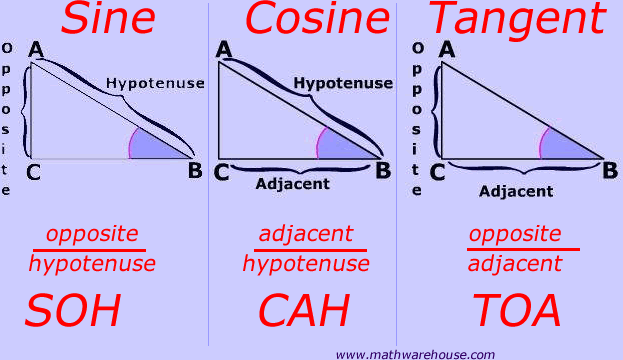
\includegraphics[width=\textwidth]{sohcahtoa}
	\end{center}
\end{frame}

\begin{frame}{Drawing a circle}
	\begin{columns}
		\begin{column}{0.48\textwidth}
			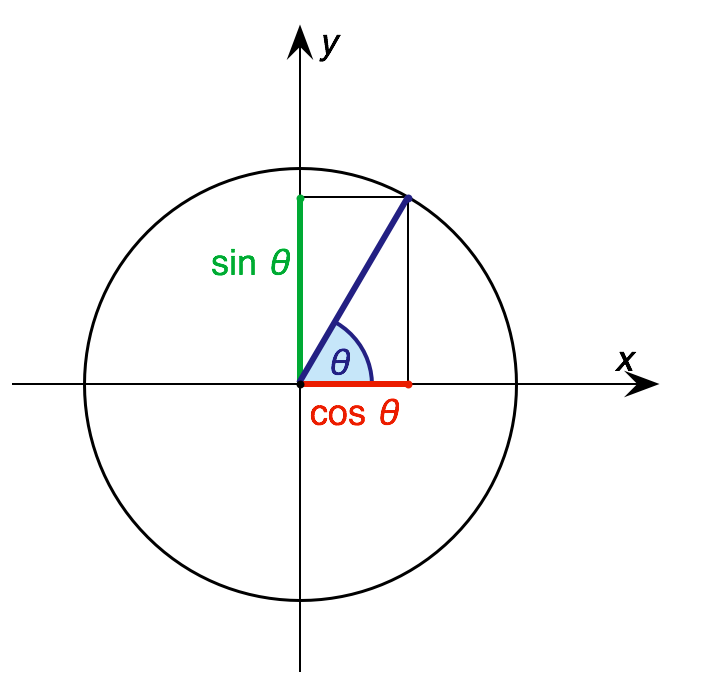
\includegraphics[width=\textwidth]{unit_circle}
		\end{column}
		\begin{column}{0.48\textwidth}
			\pause Circle of \textbf{radius} $r$
			
			\pause $\therefore$ hypotenuse = $r$
			
			\vspace{2ex}
			
			\pause $\cos \theta = \frac{\text{adjacent}}{\text{hypotenuse}} = \frac{x}{r}$
			
			\pause $\therefore x = r \cos \theta$
			
			\vspace{2ex}
			
			\pause $\sin \theta = \frac{\text{opposite}}{\text{hypotenuse}} = \frac{y}{r}$
			
			\pause $\therefore y = r \sin \theta$

			\vspace{2ex}
			
			\pause NB: this works even if $\cos \theta$ and/or $\sin \theta$ are negative
				(i.e.\ if $\theta$ is not between $0^\circ$ and $90^\circ$)
		\end{column}
	\end{columns}
\end{frame}

\begin{frame}{Drawing a cylinder}
	\begin{center}
		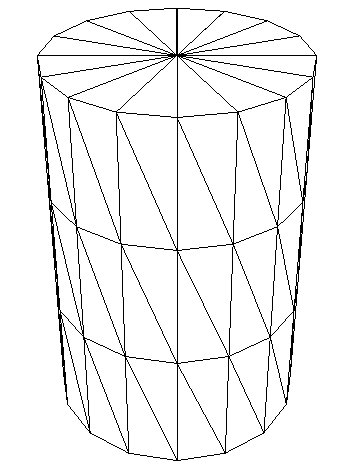
\includegraphics[height=0.8\textheight]{cylinder}
	\end{center}
\end{frame}

\begin{frame}{Drawing a sphere}
	\begin{center}
		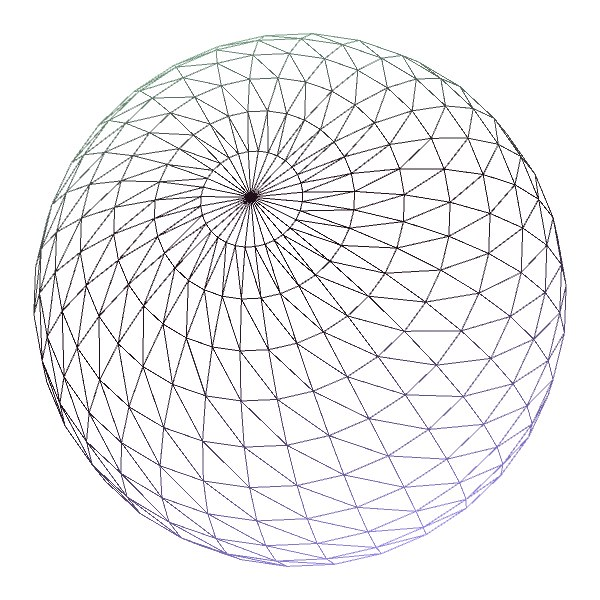
\includegraphics[height=0.8\textheight]{sphere}
	\end{center}
\end{frame}


\part{Vertices}
\frame{\partpage}

\begin{frame}{Interleaved Vertices}
	\begin{itemize}
		\pause\item Up until this point we have been storing vertex positions as floats
		\pause\item If we need a vertex to have colours, we can store these in a separate Vertex Buffer
		\pause\item Or we can create a \textbf{C structure} which represents a Vertex, which has member variables which represent positions, colours, normals etc
		\pause\item This is known as Interleaved Vertices and in \pause\textbf{MOST} cases is more efficient
	\end{itemize}
\end{frame}

\begin{frame}[fragile]{Vertex Structure 1}
	\begin{lstlisting}
		struct Vertex
		{
			float x,y,z;
		};
		
		Vertex v[]={{-0.5f,-0.5f,0.0f},
					{0.5f,-0.5f,0.0f},
					{0.0f,0.5f,0.0f}};
					 
	\end{lstlisting}
\end{frame}

\begin{frame}[fragile]{Vertex Structure 2}
	\begin{lstlisting}
		struct Vertex
		{
			float x,y,z;
			float r,g,b,a;
		};
		
		Vertex v[]={{-0.5f,-0.5f,0.0f,1.0f,0.0f,0.0f,1.0f},
					{0.5f,-0.5f,0.0f,0.0f,1.0f,0.0f,1.0f},
					{0.0f,0.5f,0.0f,0.0f,0.0f,1.0f,1.0f}};
	\end{lstlisting}
\end{frame}

\begin{frame}{Changes to the Vertex Buffer}
	\begin{itemize}
		\pause\item There will be a slight change to our vertex buffer
		\pause\item We have to take into account the size of the Vertex structure and the number of vertices in the buffer
	\end{itemize}
\end{frame}

\begin{frame}[fragile]{Vertex Buffer Changes - Old version}
	\begin{lstlisting}
		glBufferData(GL_ARRAY_BUFFER, sizeof(g_vertex_buffer_data), g_vertex_buffer_data, GL_STATIC_DRAW);
	\end{lstlisting}
\end{frame}

\begin{frame}[fragile]{Vertex Buffer Changes - new version}
	\begin{lstlisting}
		glBufferData(GL_ARRAY_BUFFER, 3* sizeof(Vertex), v, GL_STATIC_DRAW);
	\end{lstlisting}
\end{frame}

\begin{frame}{Changes to the Vertex Array}
	\begin{itemize}
		\pause\item Since the layout of the vertices have changed in memory, we need to update the Vertex Array Object to reflect this
		\pause\item Remember that the VAO describes the format of the vertices to the pipeline and enables the binding of vertex data to attributes in the shader 
	\end{itemize}
\end{frame}

\begin{frame}[fragile]{Vertex Array Object - Old version}
\begin{lstlisting}
	glEnableVertexAttribArray(0);
	glVertexAttribPointer(0,3,GL_FLOAT,GL_FALSE,0,(void*)0);
\end{lstlisting}
\end{frame}

\begin{frame}[fragile]{Vertex Array Object - New version}
\begin{lstlisting}
	glEnableVertexAttribArray(0);
	glVertexAttribPointer(0,3,GL_FLOAT,GL_FALSE,sizeof(Vertex),(void*)0);
	
	glEnableVertexAttribArray(1);
	glVertexAttribPointer(1,4,GL_FLOAT,GL_FALSE,sizeof(Vertex),(void*)(3*sizeof(float)));
\end{lstlisting}
\end{frame}

\begin{frame}{Memory and Vertex Array Object 1}
		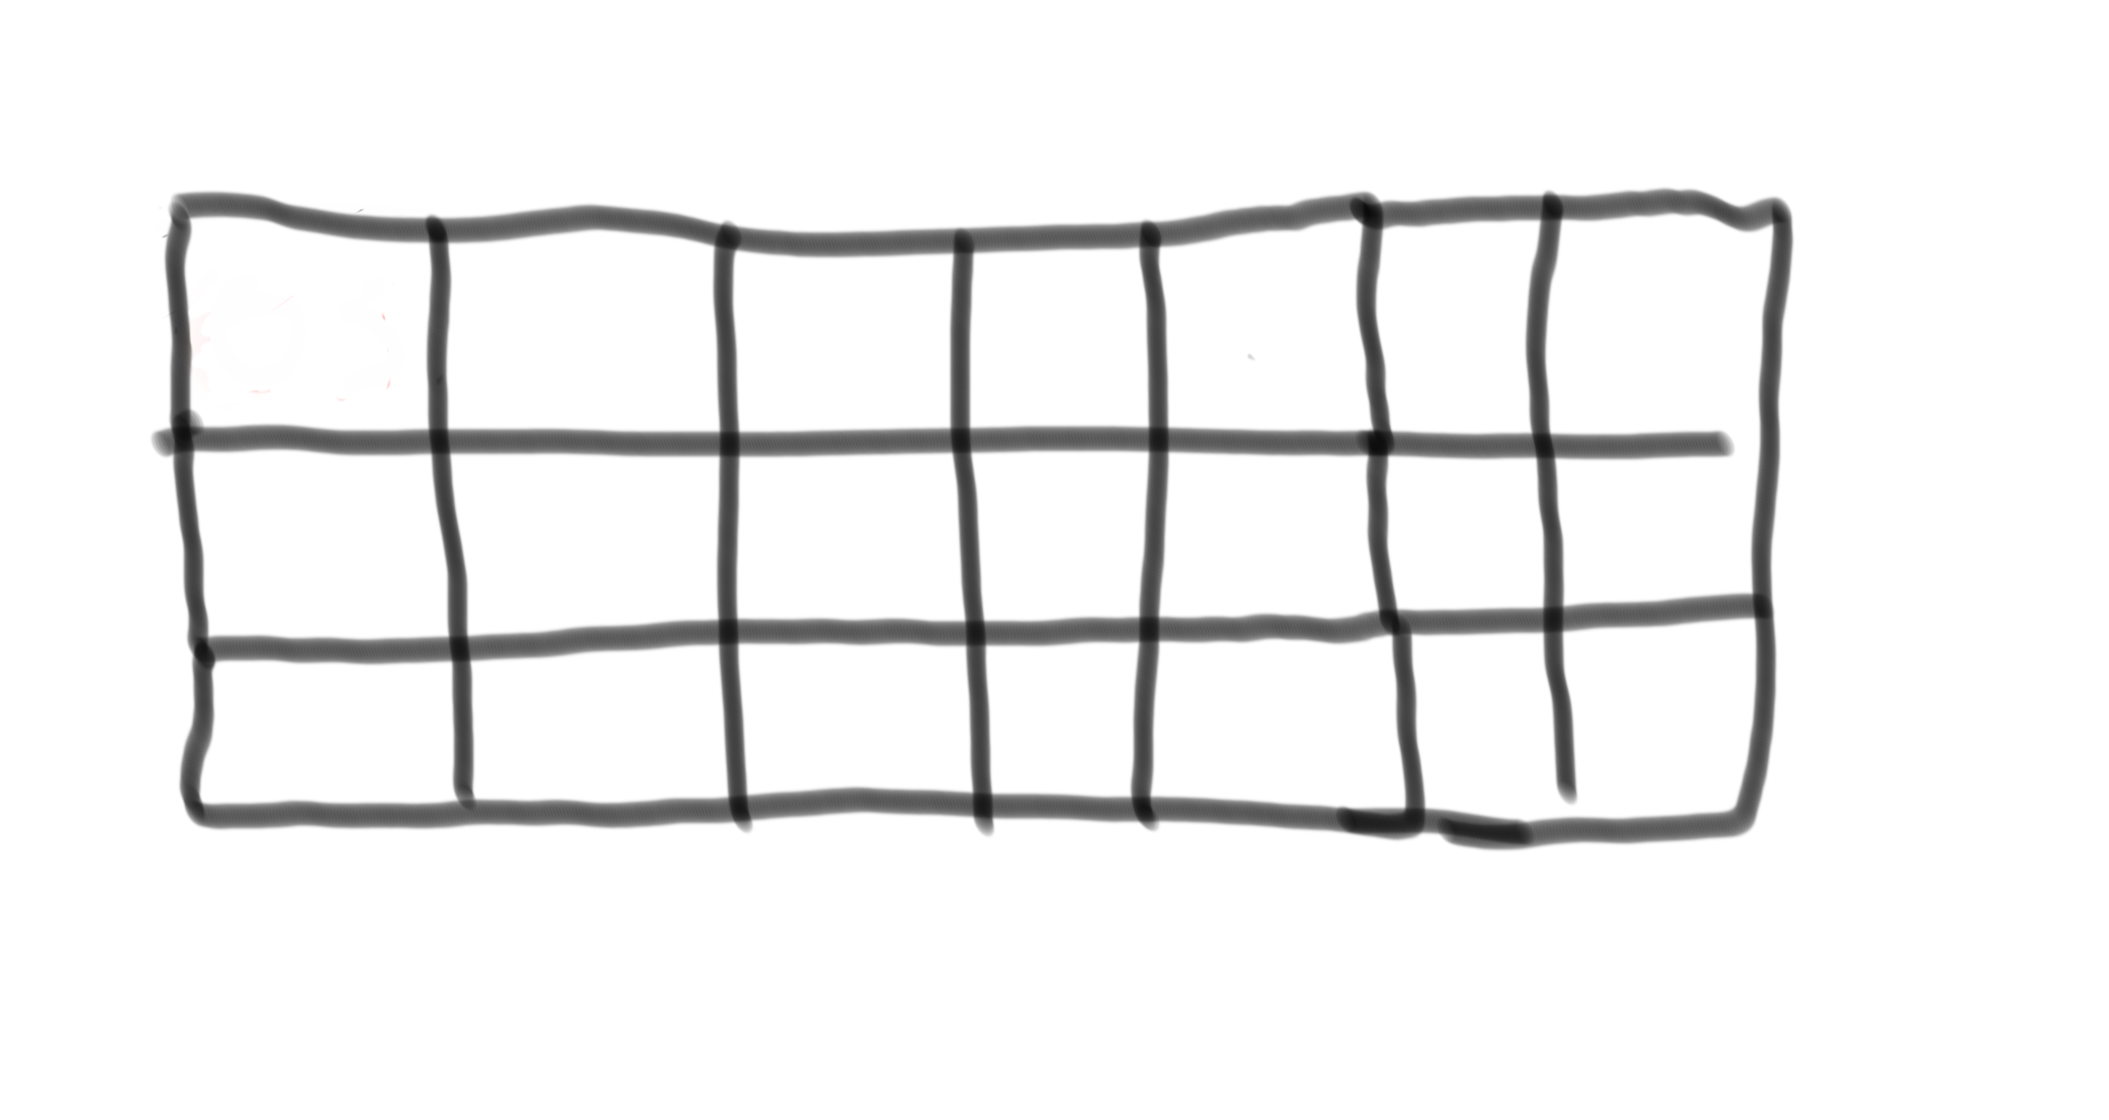
\includegraphics[height=0.8\textheight]{MemoryLayoutStarter}	
\end{frame}

\begin{frame}{Memory and Vertex Array Object 2}
	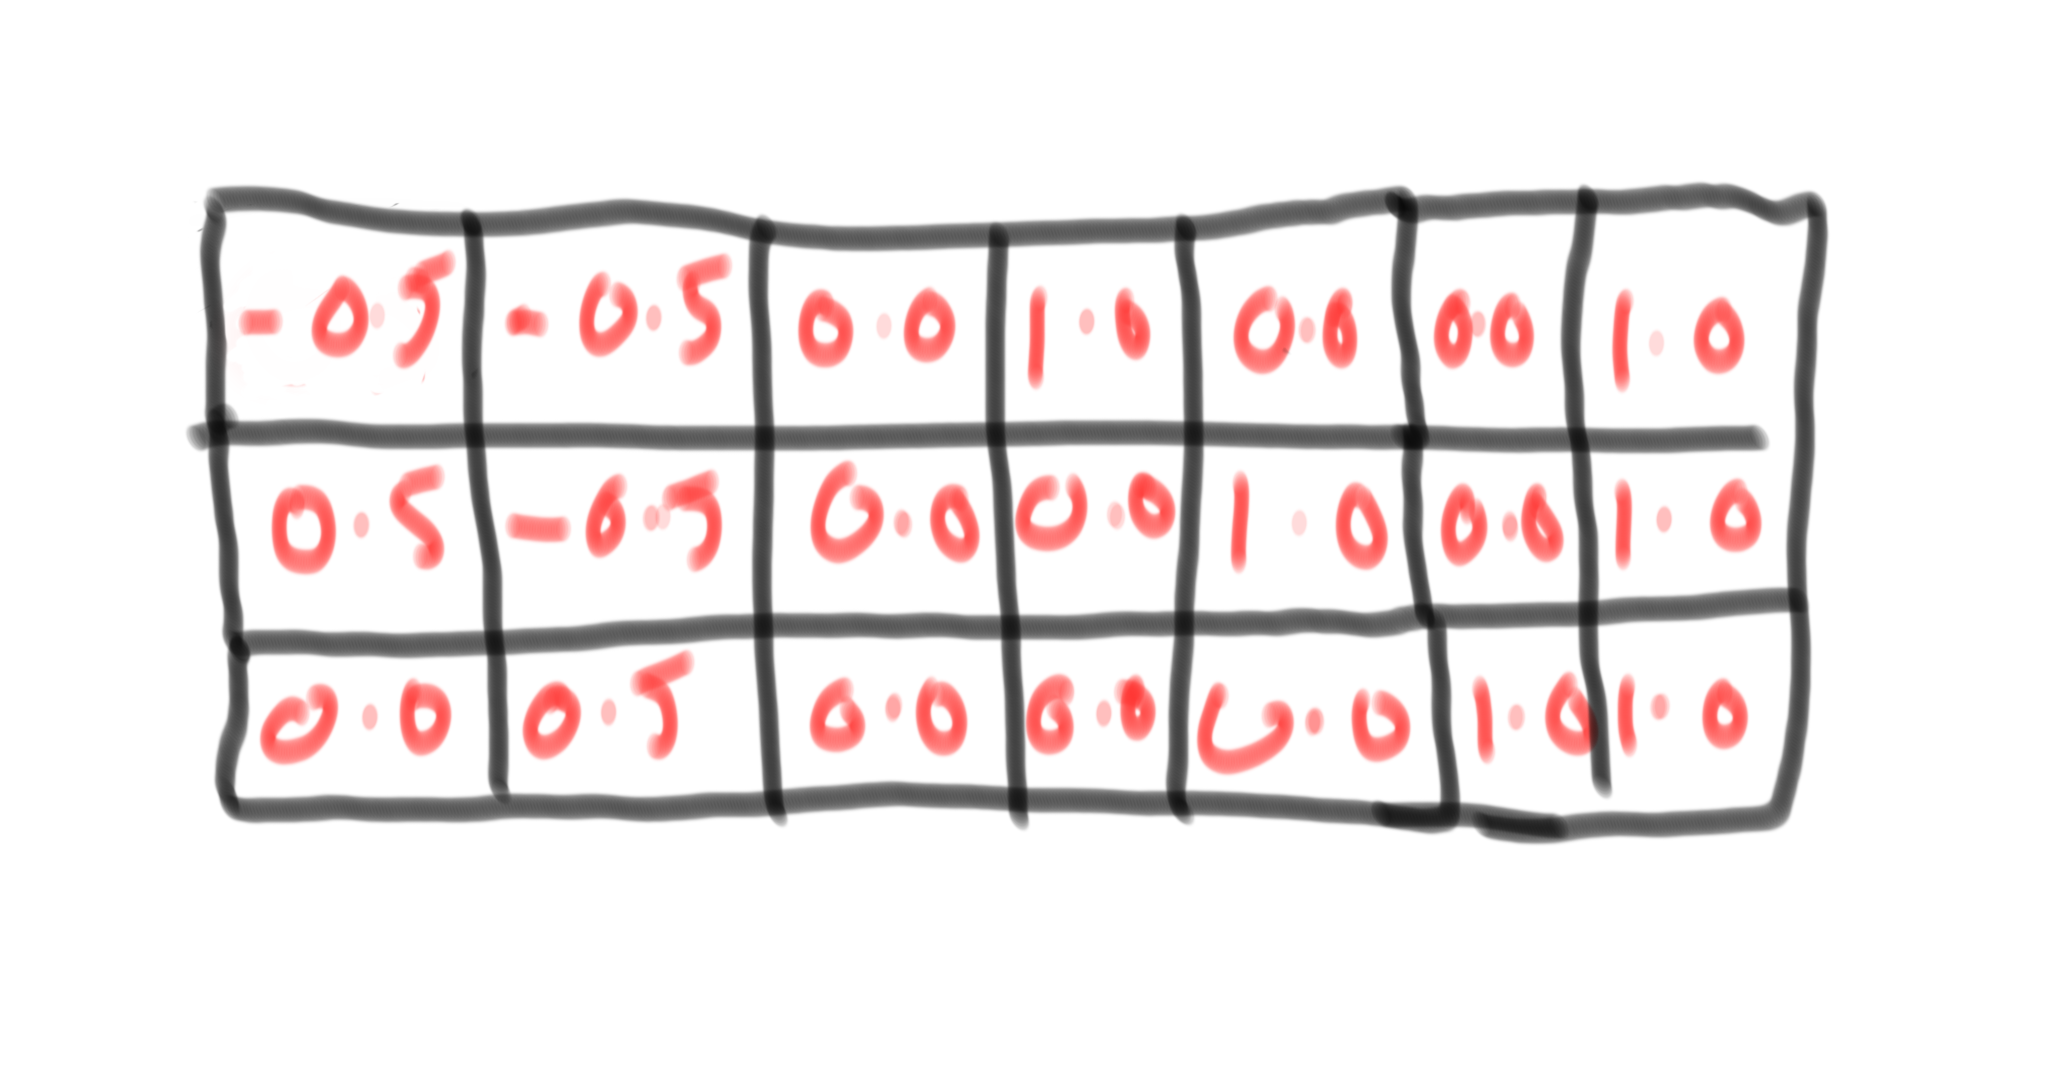
\includegraphics[height=0.8\textheight]{MemoryLayoutValues}	
\end{frame}

\begin{frame}{Memory and Vertex Array Object 3 - Stride}
	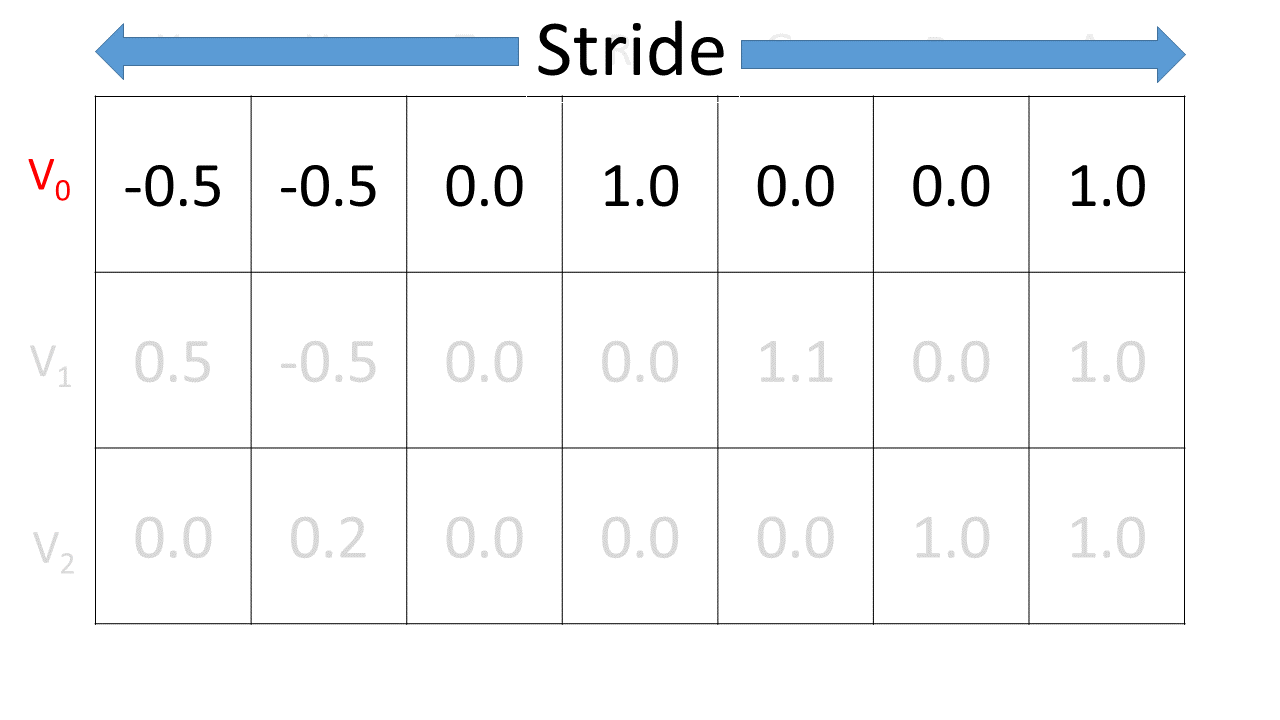
\includegraphics[height=0.8\textheight]{MemoryLayoutStride}	
\end{frame}

\begin{frame}{Memory and Vertex Array Object 3 - Offset}
	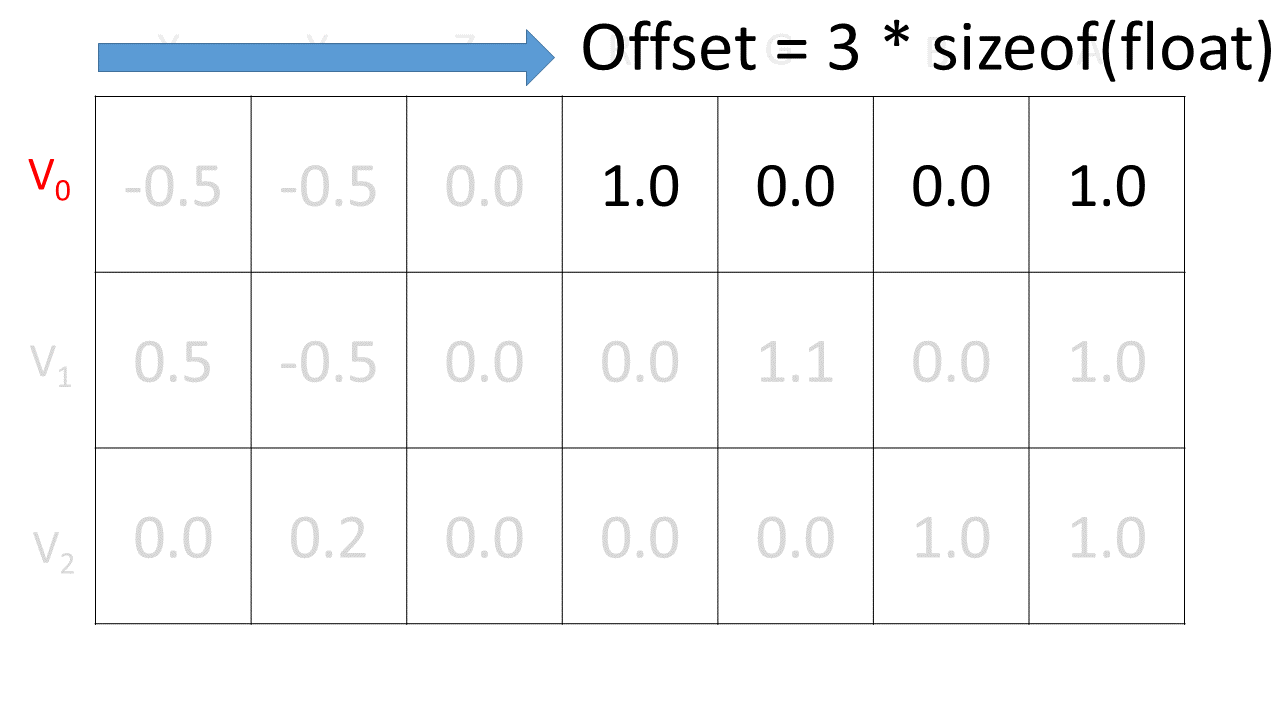
\includegraphics[height=0.8\textheight]{MemoryLayoutOffset}	
\end{frame}
\part{Indices}
\frame{\partpage}
\part{Vertex Shader}
\frame{\partpage}
\part{Fragment Shader}
\frame{\partpage}
\part{Meshes Example}
\frame{\partpage}

\begin{frame}{Unity3D - Meshes}
	\begin{itemize}
		\item Mesh Class - \url{https://docs.unity3d.com/ScriptReference/Mesh.html}
	\end{itemize}
\end{frame}

\begin{frame}{UE4 - Meshes}
	\begin{itemize}
		\item Procedural Mesh Blueprints - \url{https://docs.unrealengine.com/en-US/BlueprintAPI/Components/ProceduralMesh/index.html}
		\url{https://www.youtube.com/watch?v=dKlMEmVgbvg}
		\item Procedural Mesh C++ -
		\url{http://wlosok.cz/procedural-mesh-in-ue4-1-triangle/}
	\end{itemize}
\end{frame}

\end{document}
